\newpage
\section{Teilversuch 6: Phänomenologische Beobachtung zum anomalen Zeeman-Effekt (transversale Beobachtung)}
	\begin{figure}[!ht]
	    \centering
	   	\begin{subfigure}{0.48\textwidth}
			\centering
			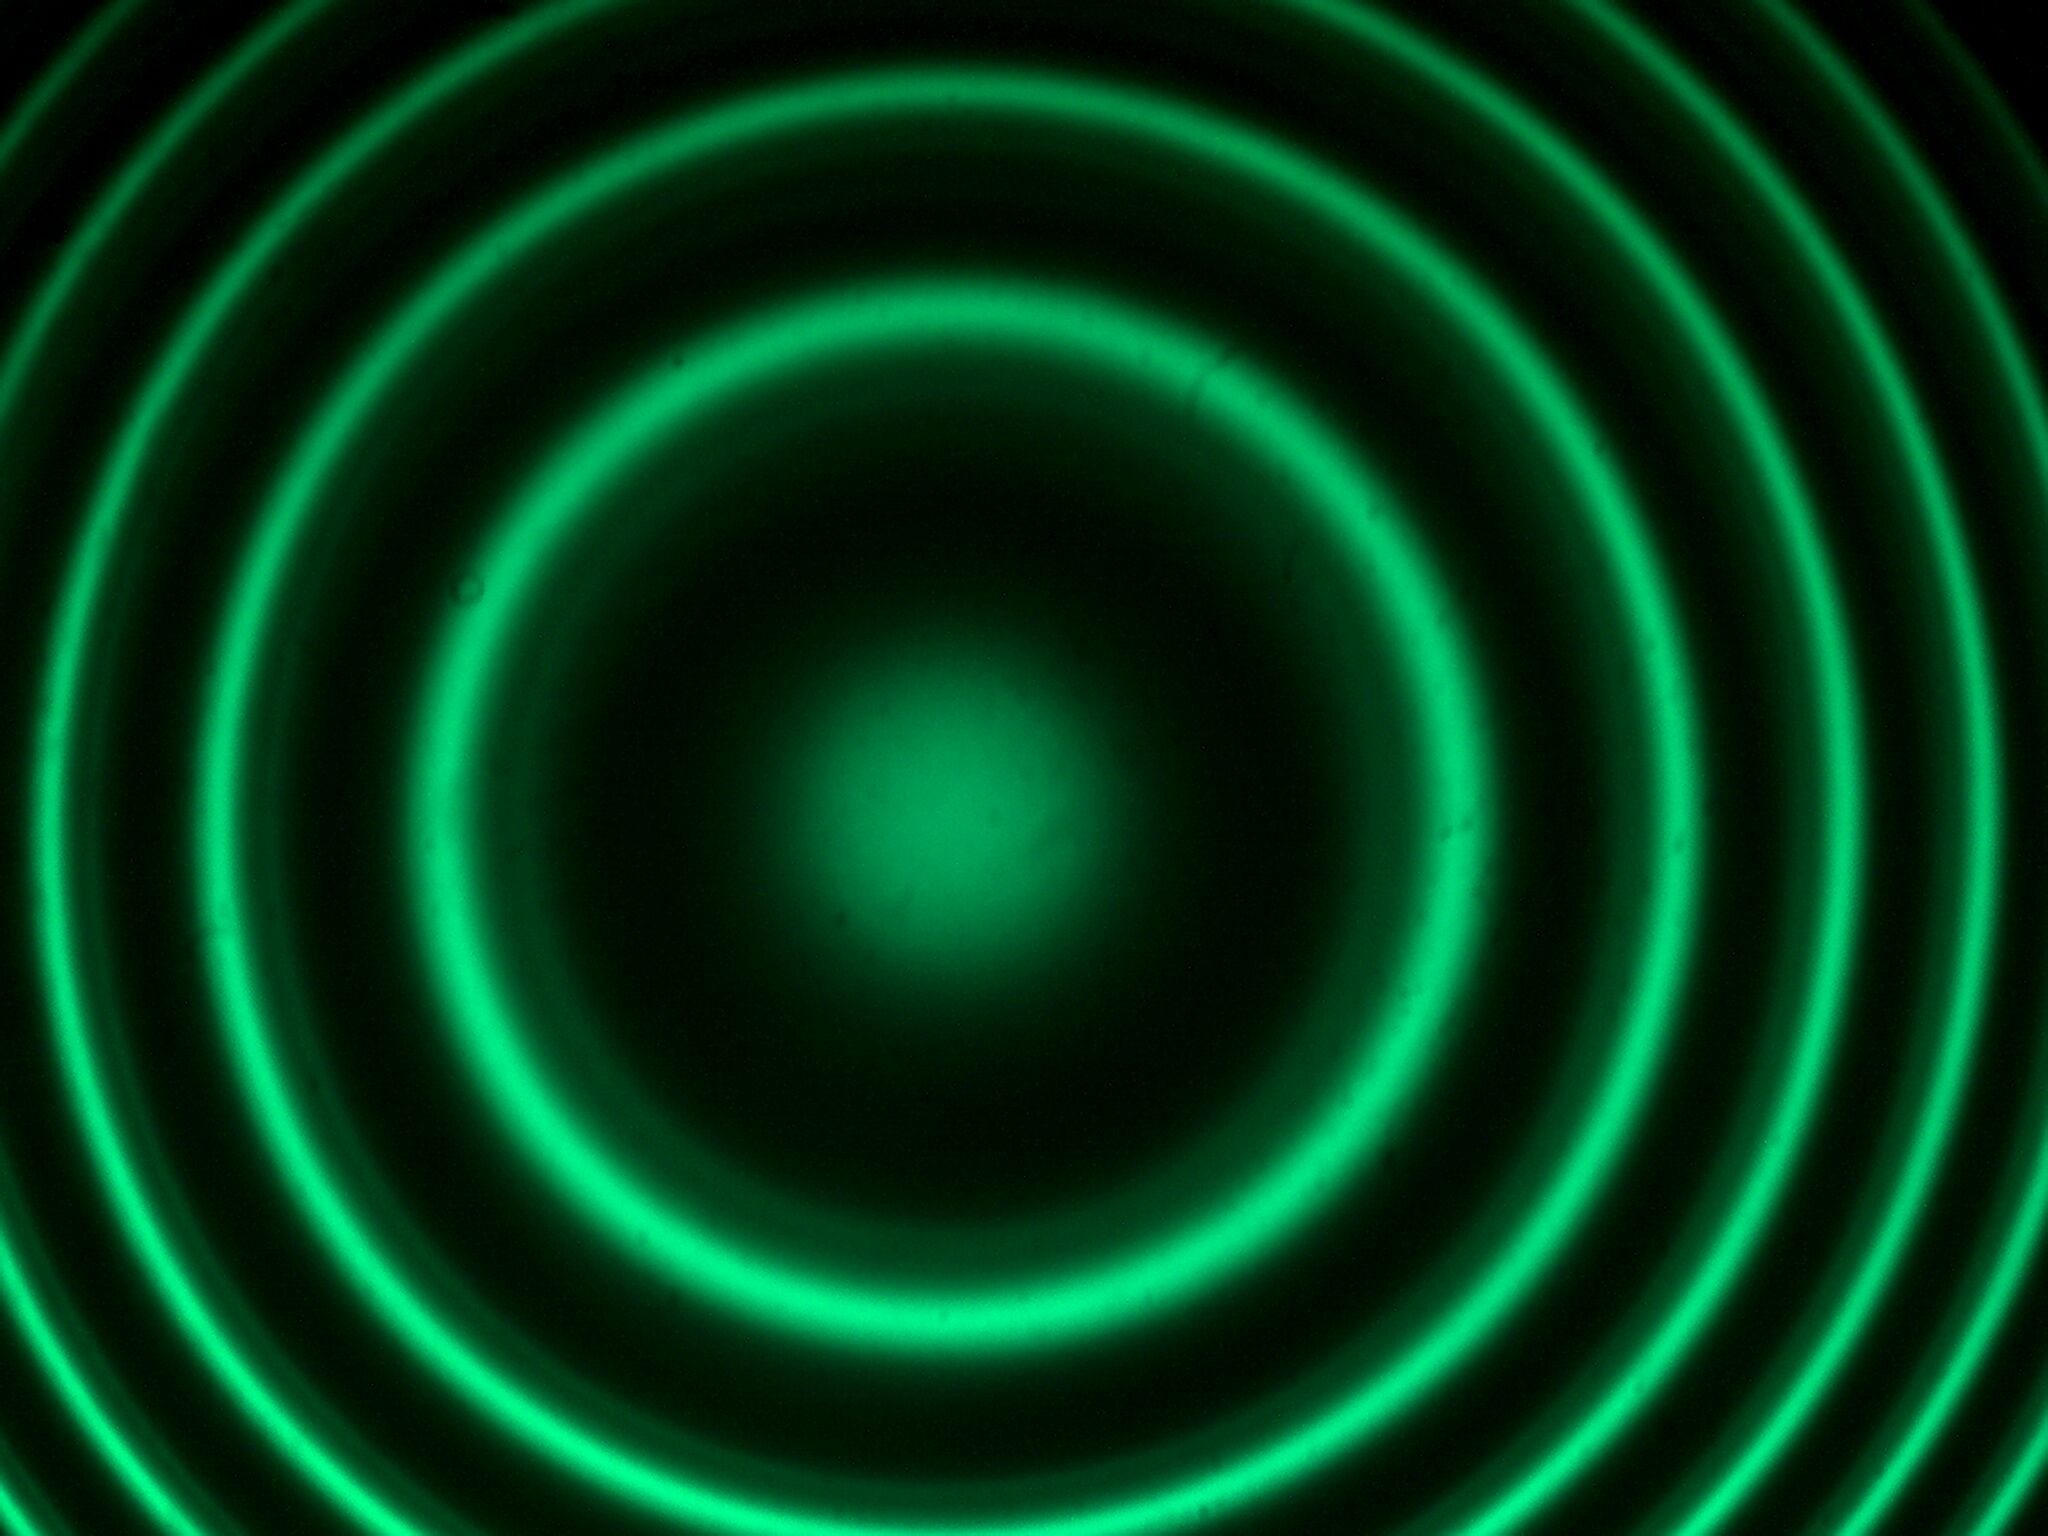
\includegraphics[width=\textwidth]{images/Capture_822.bmp.jpg}
			\caption{mit Pol-Filter}
			\vspace{0.5\baselineskip}
		\end{subfigure}
		\hfill
		\begin{subfigure}{0.48\textwidth}
			\centering
			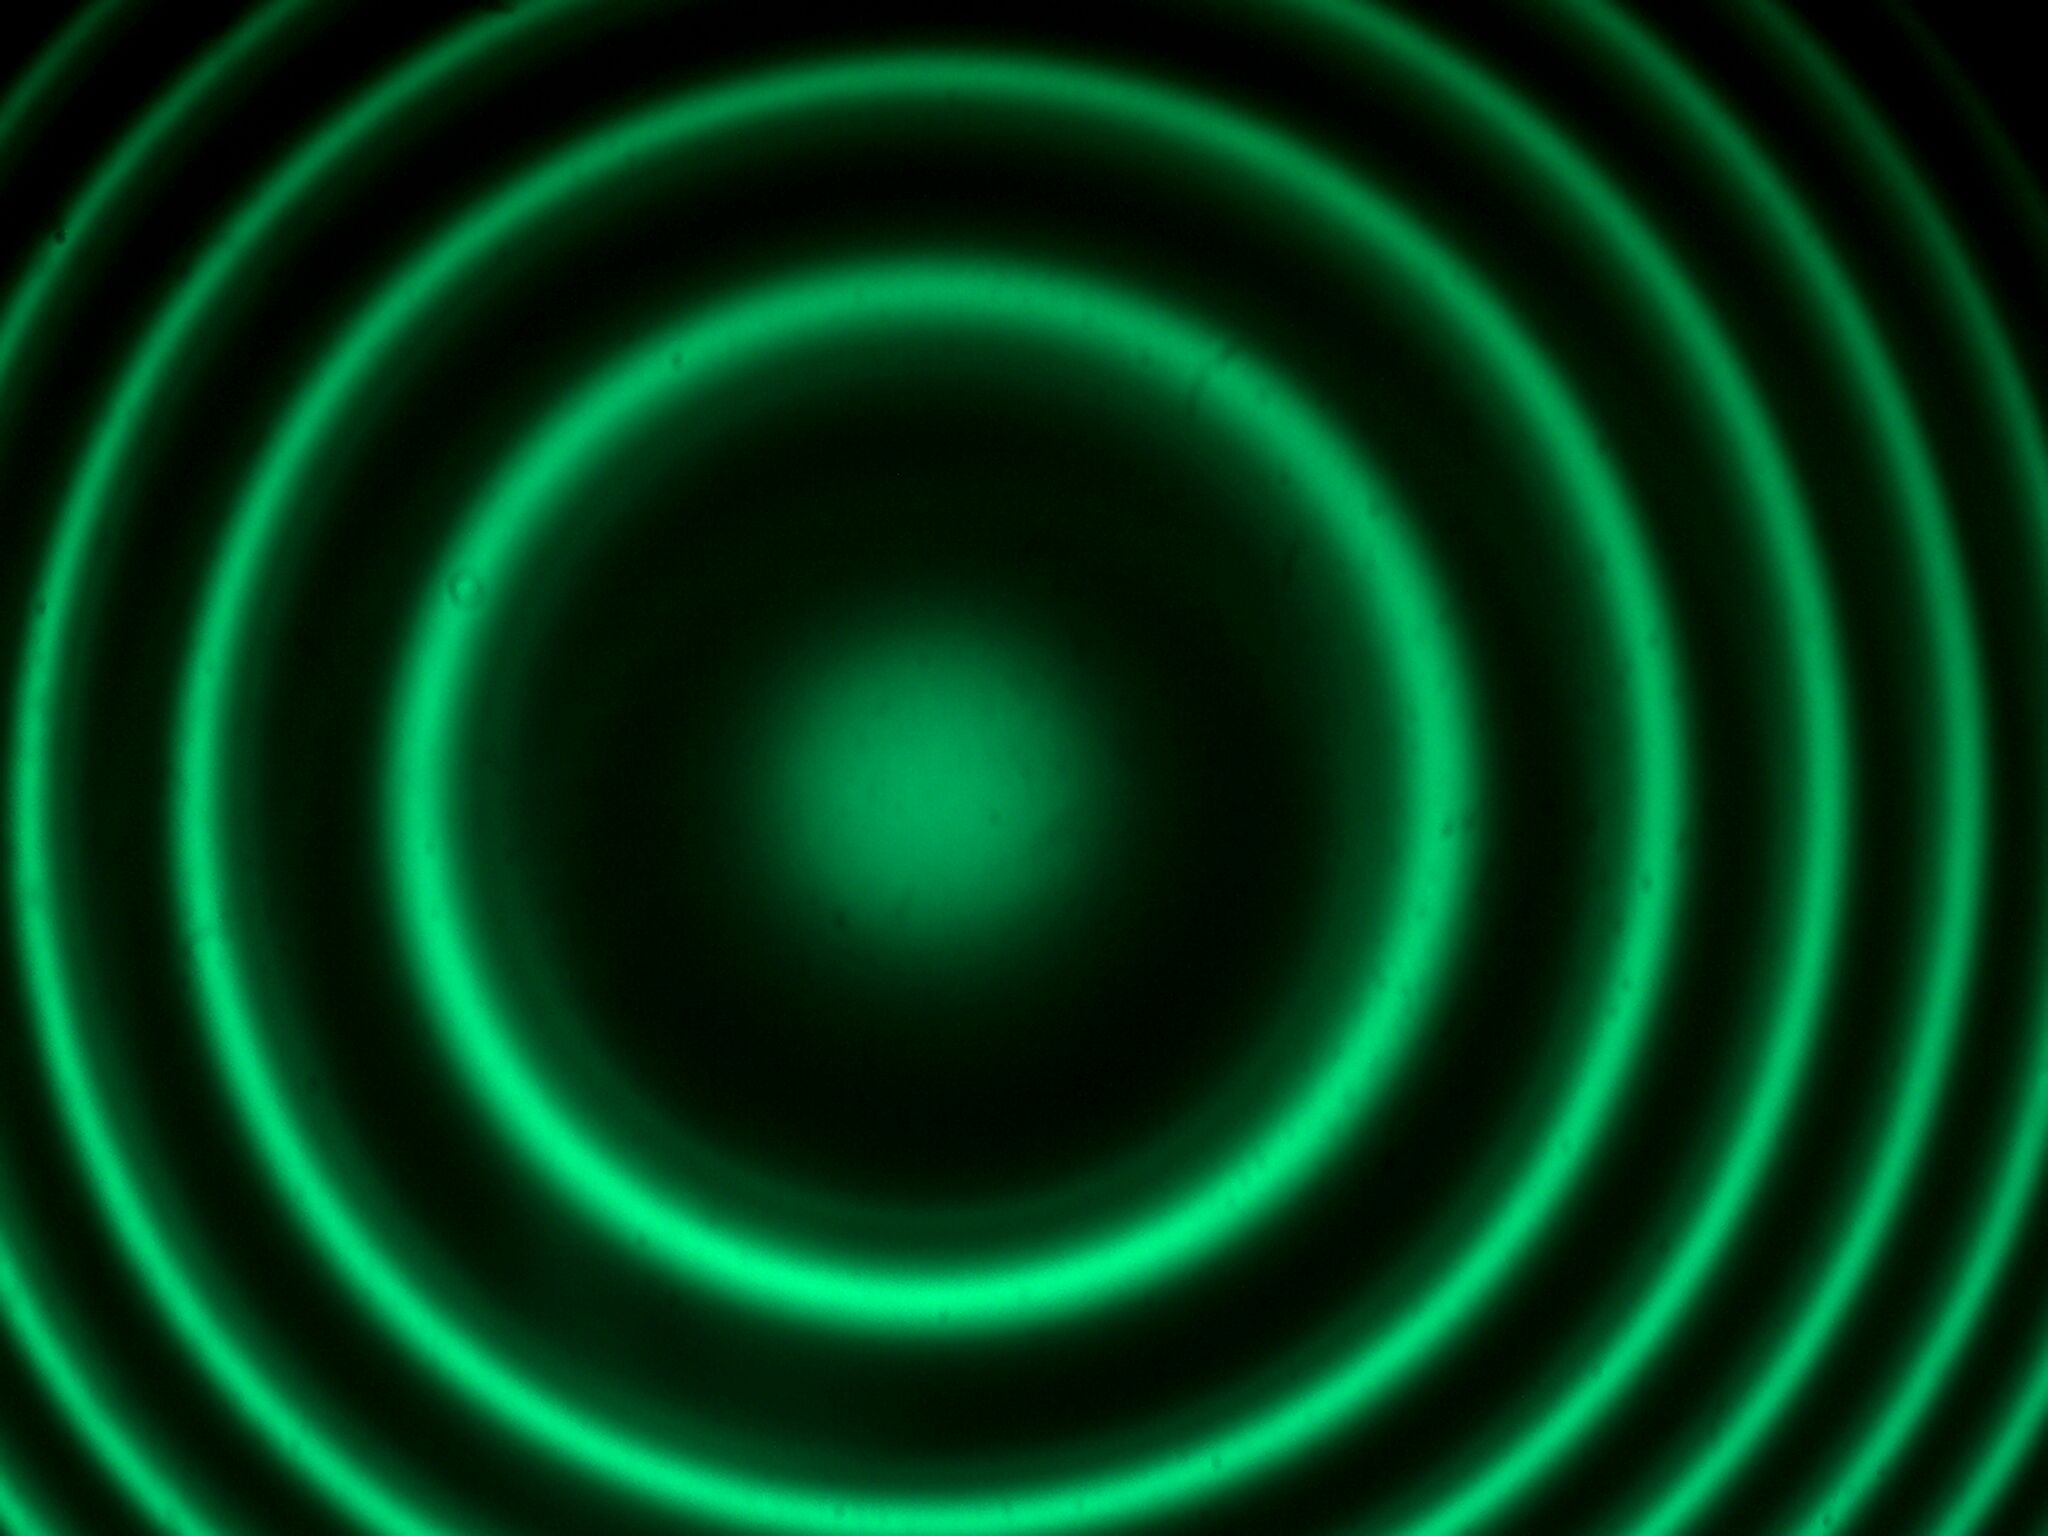
\includegraphics[width=\textwidth]{images/Capture_824.bmp.jpg}
			\caption{ohne Pol-Filter}
			\vspace{0.5\baselineskip}
		\end{subfigure}
		\begin{subfigure}{0.48\textwidth}
			\centering
			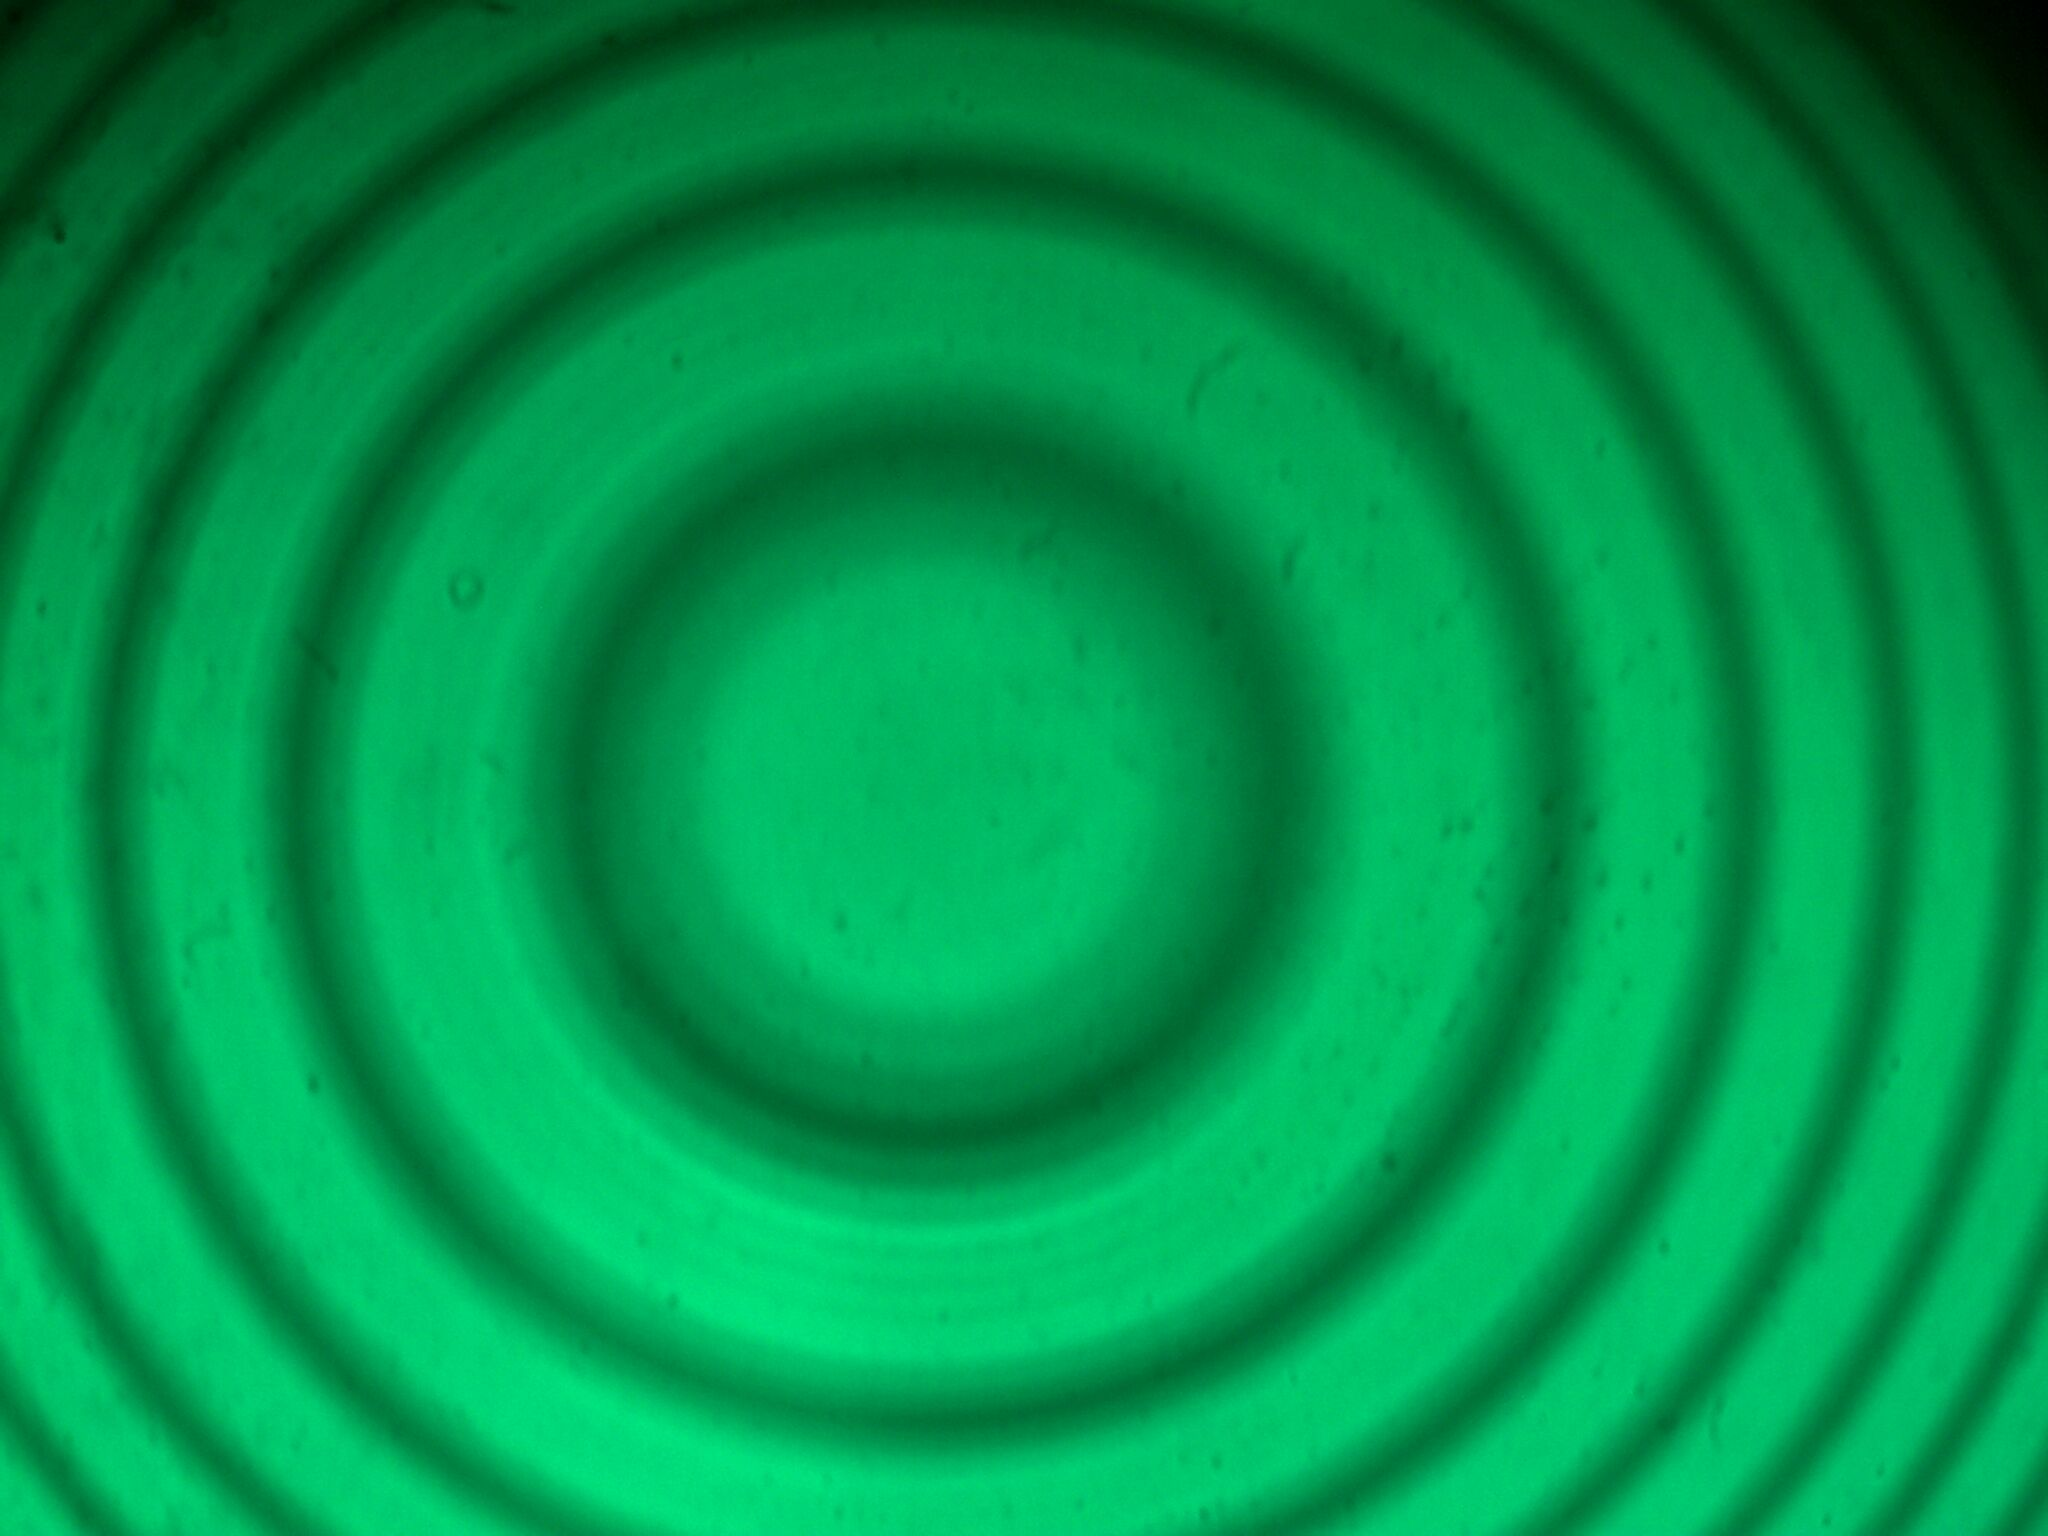
\includegraphics[width=\textwidth]{images/Capture_823.bmp.jpg}
			\caption{$I = \SI{7.45(1)}{\ampere}$}
			\vspace{0.5\baselineskip}
		\end{subfigure}
	    \caption{Teilversuch 6}
	\end{figure}